% Correcting Forward Model Mismatch in Coded Aperture Snapshot Spectral
% Imaging via Two-Stage Differentiable Calibration
%
% ECCV-style conference paper

\documentclass[runningheads]{llncs}
\usepackage[T1]{fontenc}
\usepackage{graphicx}
\usepackage{amsmath,amssymb}
\usepackage{booktabs}
\usepackage{multirow}
\usepackage{xcolor}
\usepackage{hyperref}
\usepackage{cleveref}
\usepackage{subcaption}
\usepackage{array}
\usepackage{algorithm}
\usepackage{algorithmic}

% Custom column type
\newcolumntype{C}[1]{>{\centering\arraybackslash}p{#1}}

% Color definitions
\definecolor{bestcolor}{rgb}{0.0, 0.5, 0.0}
\definecolor{worstcolor}{rgb}{0.7, 0.0, 0.0}

\newcommand{\best}[1]{\textcolor{bestcolor}{\textbf{#1}}}
\newcommand{\worst}[1]{\textcolor{worstcolor}{#1}}
\newcommand{\gain}[1]{\textcolor{bestcolor}{+#1}}

\begin{document}

\title{Correcting Forward Model Mismatch in Coded Aperture Snapshot Spectral Imaging via Two-Stage Differentiable Calibration}
\titlerunning{Differentiable CASSI Calibration}

\author{Chengshuai Yang}
\authorrunning{C. Yang}
\institute{NextGen PlatformAI C Corp}

\maketitle

% ============================================================================
% ABSTRACT
% ============================================================================
\begin{abstract}
Coded aperture snapshot spectral imaging (CASSI) captures a 3D hyperspectral cube from a single 2D measurement using a coded mask and spectral dispersion.
Deep learning reconstructors such as MST achieve state-of-the-art quality ($>$34\,dB) but assume perfect knowledge of the forward operator.
In practice, sub-pixel mask misalignment ($\Delta x$, $\Delta y$, $\theta$) and dispersion drift ($a_1$, $\alpha$) between the coded aperture and detector are unavoidable, yet even moderate mismatch degrades MST-L reconstruction by over 16\,dB.
We propose a two-stage differentiable calibration pipeline: (1)~a coarse hierarchical grid search scored by GPU-accelerated GAP-TV, followed by (2)~joint gradient refinement through an unrolled differentiable forward operator using a Straight-Through Estimator (STE) for integer dispersion offsets, plus a 1D grid search for dispersion slope recovery.
The pipeline is self-supervised, requiring only the measurement and nominal mask---no ground truth scene.
On 10 KAIST benchmark scenes with injected 5-parameter mismatch ($\Delta x{=}1.5$, $\Delta y{=}1.0$, $\theta{=}0.3^\circ$, $a_1{=}2.04$\,px/band, $\alpha{=}0.5^\circ$), our method recovers significant quality for mask-aware methods through self-supervised calibration.
We evaluate five reconstruction methods (GAP-TV, MST-S, MST-L, HDNet, PnP-HSICNN) across four scenarios, revealing a mask-sensitivity spectrum: mask-guided transformers suffer catastrophic degradation but gain most from calibration, while deep prior methods (HDNet) show inherent robustness with smaller calibration benefit.
We release all code, results, and a standardized four-scenario evaluation framework.

\keywords{CASSI \and Operator mismatch \and Differentiable calibration \and Straight-Through Estimator \and Hyperspectral imaging}
\end{abstract}

% ============================================================================
% 1. INTRODUCTION
% ============================================================================
\section{Introduction}
\label{sec:intro}

Coded aperture snapshot spectral imaging (CASSI)~\cite{wagadarikar2008cassi,arce2014cassi} captures a 3D hyperspectral cube $\mathbf{x} \in \mathbb{R}^{H \times W \times \Lambda}$ from a single 2D measurement $\mathbf{y} \in \mathbb{R}^{H \times W'}$ through the combined action of a binary coded mask and a dispersive element.
The forward model is
\begin{equation}
\label{eq:cassi_forward}
    y(i,j) = \sum_{k=1}^{\Lambda} m(i,j) \cdot x(i, j - d_k, k) + n(i,j),
\end{equation}
where $m$ is the coded aperture, $d_k = k \cdot s$ is the spectral dispersion offset for band $k$ with stride $s$, and $n$ is measurement noise.

Recent deep learning approaches---particularly Mask-guided Spectral-wise Transformers (MST)~\cite{cai2022mst,cai2022mst_pp}---achieve remarkable reconstruction quality ($>$34\,dB PSNR on the KAIST benchmark~\cite{choi2017kaist}) by jointly processing the measurement and the known mask pattern.
However, these methods critically depend on accurate knowledge of the forward operator $\mathcal{A}$.

\textbf{The mismatch problem.}
In deployed CASSI systems, the actual mask position inevitably differs from the assumed position due to manufacturing tolerances, assembly errors, and thermal drift.
Five parameters characterize the dominant misalignment: horizontal shift $\Delta x$, vertical shift $\Delta y$, and rotation angle $\theta$ for the mask, plus dispersion slope $a_1$ and axis angle $\alpha$ for the prism.
Even modest mismatches ($\Delta x = 1.5$\,px, $\Delta y = 1.0$\,px, $\theta = 0.3^\circ$, $a_1 = 2.04$\,px/band, $\alpha = 0.5^\circ$) degrade MST-L reconstruction by over 16\,dB, rendering the system effectively unusable.
In contrast, deep prior methods like HDNet~\cite{hu2022hdnet} suffer less degradation due to their learned spectral priors, while classical methods like GAP-TV~\cite{yuan2016gap} show minimal degradation but at lower peak quality.

\textbf{Challenges in CASSI calibration.}
Correcting mismatch through the reconstruction pipeline presents unique challenges:
\begin{enumerate}
    \item \textbf{Integer dispersion}: The spectral dispersion $d_k$ maps to integer pixel offsets, creating a non-differentiable forward operator.
    \item \textbf{Coupled parameters}: Translation, rotation, and dispersion drift interact through the mask pattern and spectral mapping, making sequential optimization suboptimal.
    \item \textbf{No ground truth}: In practice, neither the true mismatch parameters nor the ground truth scene are available---calibration must be self-supervised from the measurement alone.
    \item \textbf{Mixed parameter types}: Mask affine parameters ($\Delta x$, $\Delta y$, $\theta$) are amenable to gradient-based optimization, while dispersion slope $a_1$ requires discrete search due to integer rounding.
\end{enumerate}

\textbf{Contributions.} We address these challenges with:
\begin{enumerate}
    \item A \textbf{differentiable CASSI forward model} using a Straight-Through Estimator (STE)~\cite{bengio2013ste} for integer dispersion offsets, enabling gradient-based calibration.
    \item A \textbf{two-stage calibration pipeline}: coarse grid search (Stage~0--1) followed by gradient refinement (Stage~2A--2C) for mask affine recovery, plus 1D grid search for dispersion slope $a_1$.
    \item A \textbf{self-supervised objective}: measurement residual minimization requires only the measurement $\mathbf{y}$ and nominal mask $\mathbf{m}$---no ground truth scene or external calibration targets.
    \item A \textbf{four-scenario evaluation framework} (Ideal, Assumed, Corrected, Oracle) that systematically quantifies mismatch degradation, calibration recovery, and residual gap across reconstruction methods.
\end{enumerate}

% ============================================================================
% 2. RELATED WORK
% ============================================================================
\section{Related Work}
\label{sec:related}

\textbf{CASSI reconstruction.}
Classical approaches including GAP-TV~\cite{yuan2016gap,meng2020gap} use alternating projection with total variation regularization.
Plug-and-play methods such as PnP-HSICNN~\cite{yuan2020pnpcassi} combine optimization frameworks (ADMM/GAP) with learned denoisers.
Deep learning methods have significantly advanced quality: HDNet~\cite{hu2022hdnet} uses dual-domain deep unfolding, while MST~\cite{cai2022mst} introduces mask-guided spectral-wise attention achieving 35+\,dB on KAIST.
All assume perfect forward operator knowledge.

\textbf{Operator-aware reconstruction.}
Physics-based learned design~\cite{kellman2019physics} optimizes optical elements end-to-end but requires differentiable forward models.
Deep unrolling approaches~\cite{ongie2020deep,zheng2021deep} embed the forward operator into network layers, making them sensitive to operator errors.
HyperReconNet~\cite{wang2019hyperreconnet} jointly optimizes mask design and reconstruction but does not address post-fabrication calibration.

\textbf{Self-calibration in computational imaging.}
Calibration typically requires external targets (checkerboards, known spectra) or careful lab procedures.
Self-calibration from measurements alone has been explored for phase retrieval~\cite{metzler2018prdeep} but not for CASSI mismatch correction with deep reconstructors.

Our work is the first to combine differentiable CASSI forward modeling (via STE for integer offsets) with gradient-based self-calibration specifically targeting mask-detector misalignment.

% ============================================================================
% 3. PROBLEM FORMULATION
% ============================================================================
\section{Problem Formulation}
\label{sec:formulation}

\subsection{CASSI Forward Model}

The SD-CASSI (single-disperser) forward model maps a hyperspectral cube $\mathbf{x} \in \mathbb{R}^{H \times W \times \Lambda}$ to a 2D measurement $\mathbf{y} \in \mathbb{R}^{H \times (W + (\Lambda-1)s)}$:
\begin{equation}
\label{eq:forward}
    \mathbf{y} = \mathcal{A}(\mathbf{x}; \mathbf{m}, \{d_k\}) = \sum_{k=1}^{\Lambda} \text{shift}_{d_k}(\mathbf{m} \odot \mathbf{x}_k) + \mathbf{n},
\end{equation}
where $\mathbf{m} \in \{0,1\}^{H \times W}$ is the coded aperture, $d_k = k \cdot s$ is the integer dispersion offset for band $k$, $s$ is the stride (typically 2), and $\text{shift}_{d_k}$ shifts the column index by $d_k$ pixels.

\subsection{Mismatch Parameterization}

We model CASSI operator mismatch as a 5-parameter perturbation combining mask misalignment and dispersion drift:
\begin{equation}
\label{eq:mismatch}
    \tilde{\mathbf{m}} = \mathcal{W}(\mathbf{m}; \Delta x, \Delta y, \theta), \quad \tilde{d}_k = a_1 \cdot k \cdot \cos\alpha, \quad \tilde{d}_k^y = a_1 \cdot k \cdot \sin\alpha,
\end{equation}
where $\mathcal{W}$ applies bilinear-interpolated translation $(\Delta x, \Delta y)$ and rotation $\theta$ about the mask center, $a_1$ is the actual dispersion slope (nominal $s = 2.0$\,px/band), and $\alpha$ is the dispersion axis angular offset.
The true measurement uses the misaligned mask $\tilde{\mathbf{m}}$ with dispersion slope $a_1$, while reconstruction assumes the nominal mask $\mathbf{m}$ with stride $s$.

\subsection{Calibration Objective}

Given measurement $\mathbf{y}$ (generated with unknown true mismatch $\boldsymbol{\psi}^* = (\Delta x^*, \Delta y^*, \theta^*, a_1^*, \alpha^*)$) and nominal mask $\mathbf{m}$, we seek:
\begin{equation}
\label{eq:objective}
    \hat{\boldsymbol{\psi}} = \arg\min_{\boldsymbol{\psi}} \left\| \mathbf{y} - \mathcal{A}\big(\mathcal{R}(\mathbf{y}, \mathcal{W}(\mathbf{m}; \boldsymbol{\psi})); \mathcal{W}(\mathbf{m}; \boldsymbol{\psi}), \{d_k\}\big) \right\|^2,
\end{equation}
where $\mathcal{R}(\mathbf{y}, \tilde{\mathbf{m}})$ is a reconstruction algorithm (GAP-TV in our pipeline) that produces a spectral cube estimate from measurement $\mathbf{y}$ using mask $\tilde{\mathbf{m}}$.
This is self-supervised: minimizing the measurement residual requires no ground truth.

% ============================================================================
% 4. METHOD
% ============================================================================
\section{Method}
\label{sec:method}

\subsection{Differentiable CASSI Forward Model}

The key challenge is that dispersion offsets $d_k = k \cdot s$ are integers, making $\text{shift}_{d_k}$ non-differentiable.
We address this with a Straight-Through Estimator (STE)~\cite{bengio2013ste}:
\begin{equation}
\label{eq:ste}
    \hat{d}_k = \text{round}(d_k), \quad \frac{\partial \hat{d}_k}{\partial d_k} \equiv 1.
\end{equation}
In the forward pass, offsets are rounded to integers for exact indexing; in the backward pass, gradients flow through as if rounding were the identity function.
This enables gradient-based optimization of parameters that influence the dispersion model.

The differentiable mask warping $\mathcal{W}(\mathbf{m}; \boldsymbol{\psi})$ uses PyTorch's \texttt{affine\_grid} and \texttt{grid\_sample} with bilinear interpolation, providing exact gradients for $\Delta x$, $\Delta y$, and $\theta$.
The sign convention matches scipy exactly: $t_x = -2\Delta x / W$, $t_y = -2\Delta y / H$.

\subsection{Differentiable GAP-TV Solver}

We unroll $K$ iterations of GAP-TV into a differentiable computation graph:
\begin{align}
    \mathbf{r}^{(t)} &= \mathbf{y} - \mathcal{A}(\mathbf{x}^{(t)}; \tilde{\mathbf{m}}, \{d_k\}), \\
    \mathbf{x}^{(t+1)} &= \text{TV}_\sigma\big(\mathbf{x}^{(t)} + \mathcal{A}^\dagger(\mathbf{r}^{(t)})\big),
\end{align}
where $\text{TV}_\sigma$ denotes Gaussian-weighted TV denoising (replacing the standard TV proximal step for differentiability), and $\mathcal{A}^\dagger$ is the adjoint (back-projection) operator.
Gradient checkpointing reduces memory from $O(K)$ to $O(\sqrt{K})$.

\subsection{Two-Stage Calibration Pipeline}

\textbf{Stage 0: Coarse 3D Grid Search.}
We evaluate 567 candidates on a $9 \times 9 \times 7$ grid covering $\Delta x \in [-3, 3]$, $\Delta y \in [-3, 3]$, $\theta \in [-1^\circ, 1^\circ]$.
Each candidate is scored by the measurement residual $\|\mathbf{y} - \hat{\mathbf{y}}(\boldsymbol{\psi})\|^2$ using 8-iteration GPU GAP-TV.

\textbf{Stage 1: Fine 3D Grid.}
Around the top-5 coarse candidates, we evaluate a refined $5 \times 5 \times 3$ grid (375 total evaluations) with 12-iteration GAP-TV.

\textbf{Stage 2A--2C: Gradient Refinement.}
Starting from the best grid candidate, we apply Adam optimization through the differentiable pipeline:
\begin{itemize}
    \item \textbf{2A}: Optimize $\Delta x$ only (50 steps, lr=0.05, $\sigma=0.5$)
    \item \textbf{2B}: Optimize $\Delta y, \theta$ (60 steps, lr=0.03/0.01, $\sigma=1.0$)
    \item \textbf{2C}: Joint refinement of all three (80 steps, lr=0.01/0.01/0.005, $\sigma=0.7$)
\end{itemize}
Cosine annealing learning rate schedule and gradient clipping ($\|g\| \leq 0.5$) stabilize optimization.
The staged approach avoids local minima from coupled parameters.

\textbf{Dispersion Slope Recovery.}
After mask affine calibration, we perform a 1D grid search over $a_1 \in \{1.90, 1.92, \ldots, 2.10\}$ (11 candidates), evaluating the measurement residual for each candidate using the calibrated mask.
The best $a_1$ is selected by minimum residual.

\textbf{Final Selection.}
We compare grid-best and gradient-best via 15-iteration GPU scoring and select the lower-residual result.

% ============================================================================
% 5. EXPERIMENTS
% ============================================================================
\section{Experiments}
\label{sec:experiments}

\subsection{Setup}

\textbf{Dataset.} 10 KAIST benchmark scenes~\cite{choi2017kaist} ($256 \times 256 \times 28$), widely used for CASSI evaluation.

\textbf{Mask.} TSA real mask from the MST benchmark suite~\cite{cai2022mst}.

\textbf{Mismatch injection.} Fixed 5-parameter mismatch: $\Delta x = 1.5$\,px, $\Delta y = 1.0$\,px, $\theta = 0.3^\circ$ (mask affine), $a_1 = 2.04$\,px/band (dispersion slope, nominal 2.0), $\alpha = 0.5^\circ$ (dispersion axis offset).
This represents moderate but realistic misalignment in deployed systems, combining mask assembly errors with optical dispersion drift.

\textbf{Noise model.} Poisson ($\alpha = 10^5$) + Gaussian ($\sigma = 0.01$).

\textbf{Reconstruction methods.}
We evaluate five methods spanning classical, plug-and-play, deep unfolding, and mask-guided transformer architectures:
\begin{itemize}
    \item \textbf{GAP-TV}~\cite{yuan2016gap}: Classical iterative, 50 iterations, $\lambda = 0.01$, stride-2. Mask-aware.
    \item \textbf{MST-S}~\cite{cai2022mst}: Mask-guided Spectral-wise Transformer, small variant (0.93M params). Mask-aware.
    \item \textbf{MST-L}~\cite{cai2022mst}: Mask-guided Spectral-wise Transformer, large variant (2.03M params). Mask-aware.
    \item \textbf{HDNet}~\cite{hu2022hdnet}: Dual-domain deep unfolding network (2.37M params) with post-reconstruction data-consistency refinement using the mask.
    \item \textbf{PnP-HSICNN}~\cite{yuan2020pnpcassi}: ADMM framework with HSI-SDeCNN deep spectral denoiser (7-channel context, sigma-conditional). 89 TV + 35 deep denoiser iterations. Mask-aware.
\end{itemize}

\textbf{Four-scenario protocol.}
\begin{enumerate}
    \item[\textbf{I}] \textbf{Ideal}: Clean measurement + ideal mask (upper bound).
    \item[\textbf{II}] \textbf{Assumed}: Corrupted measurement + ideal mask (baseline degradation).
    \item[\textbf{III}] \textbf{Corrected}: Corrupted measurement + calibrated mask (our method).
    \item[\textbf{IV}] \textbf{Oracle}: Corrupted measurement + truth mask (oracle recovery).
\end{enumerate}

\subsection{Main Results}

\Cref{tab:main_results} presents reconstruction quality across four scenarios for all five methods.
Key findings:

\textbf{Mask-guided methods suffer catastrophic degradation.}
MST-L drops 16.72\,dB from Scenario~I (34.81) to II (18.09), and MST-S drops 15.97\,dB (33.98$\to$18.01).
In contrast, HDNet degrades by only 10.47\,dB (34.66$\to$24.18) because its learned spectral prior provides inherent robustness to mask mismatch.
GAP-TV (classical) shows only 0.42\,dB degradation.
This reveals a \emph{mask-sensitivity spectrum}: methods that rely more heavily on the mask during reconstruction are more sensitive to mismatch.

\textbf{Calibration recovers significant quality for mask-aware methods.}
Our two-stage pipeline (Scenario~III) recovers +3.46\,dB for MST-S, +3.45\,dB for MST-L, and +2.21\,dB for PnP-HSICNN.
The residual gap between III and IV (oracle) is 2.65--2.85\,dB for MST-S/L, indicating that most of the recoverable quality is captured by our calibration.

\textbf{Deep prior methods show robustness but limited calibration benefit.}
HDNet achieves the best Scenario~II performance (24.18\,dB) despite using only lightweight data-consistency refinement with the mask.
Its small calibration gain (+0.06\,dB) confirms that the learned prior dominates the mask-based update, making it naturally robust but unable to leverage improved mask estimates.

\textbf{PnP-HSICNN benefits substantially from calibration.}
The ADMM-based plug-and-play method recovers +2.21\,dB (14.92$\to$17.13), with its oracle gain of +5.97\,dB demonstrating strong mask-dependence.

\Cref{fig:scenario_comparison} visualizes the PSNR distribution across scenarios and methods.

\begin{figure}[t]
\centering

\includegraphics[width=\linewidth]{figures/fig3_scenario_comparison.pdf}
\caption{Grouped bar chart of reconstruction quality (PSNR) across four scenarios for five methods on 10 KAIST scenes. Mask-guided methods (MST-S/L) show largest degradation (I$\to$II) and calibration gain (II$\to$III), while HDNet is most robust to mismatch.}
\label{fig:scenario_comparison}
\end{figure}

\begin{table}[t]
\centering
\caption{Reconstruction quality (PSNR in dB, mean$\pm$std) across four scenarios on 10 KAIST scenes. 5-parameter mismatch: $\Delta x{=}1.5$, $\Delta y{=}1.0$, $\theta{=}0.3^\circ$, $a_1{=}2.04$, $\alpha{=}0.5^\circ$. Degradation = I$-$II. Gain = III$-$II.}
\label{tab:main_results}
\small
\setlength{\tabcolsep}{3.5pt}
\begin{tabular}{l ccccc c}
\toprule
Method & Sc.~I & Sc.~II & Sc.~III & Sc.~IV & Degrad. & Gain \\
 & (Ideal) & (Assumed) & (Corrected) & (Oracle) & (I$\to$II) & (II$\to$III) \\
\midrule
GAP-TV & 20.37$\pm$1.84 & 19.95$\pm$1.78 & 20.43$\pm$1.74 & 21.20$\pm$1.74 & $-$0.42 & \textbf{+0.48}$\pm$0.19 \\
MST-S  & 33.98$\pm$2.50 & 18.01$\pm$2.14 & 21.47$\pm$2.53 & 24.12$\pm$2.03 & $-$15.97 & \textbf{+3.46}$\pm$0.97 \\
MST-L  & \best{34.81$\pm$2.11} & 18.09$\pm$1.97 & 21.54$\pm$2.34 & 24.39$\pm$2.02 & $-$16.72 & \textbf{+3.45}$\pm$1.01 \\
HDNet  & 34.66$\pm$2.62 & \best{24.18$\pm$2.86} & \best{24.24$\pm$2.84} & 24.26$\pm$2.85 & $-$10.47 & \textbf{+0.06}$\pm$0.04 \\
PnP-HSICNN & 21.70$\pm$6.16 & 14.92$\pm$2.28 & 17.13$\pm$3.15 & 20.89$\pm$4.51 & $-$6.78 & \textbf{+2.21}$\pm$2.10 \\
\bottomrule
\end{tabular}
\vspace{-2mm}
\end{table}

\subsection{Parameter Recovery}

\Cref{tab:param_recovery} shows aggregated mismatch parameter recovery statistics across all five parameters (\Cref{fig:param_recovery} visualizes per-scene estimates).
The mask affine parameters ($\Delta x$, $\Delta y$, $\theta$) are recovered via gradient refinement with RMSE of 0.667\,px, 0.564\,px, and 0.768$^\circ$ respectively.
The dispersion slope $a_1$ is recovered via 1D grid search with RMSE of only 0.134\,px/band.
The dispersion axis angle $\alpha$ has negligible effect at native resolution (vertical offsets round to zero for $|\alpha| < 2^\circ$ with 28 bands) and is not actively estimated.

\begin{figure}[t]
\centering

\includegraphics[width=\linewidth]{figures/fig5_parameter_recovery.pdf}
\caption{Per-scene estimated vs.\ true mismatch parameters across 10 KAIST scenes. Dashed lines indicate ground truth values ($\Delta x{=}1.5$, $\Delta y{=}1.0$, $\theta{=}0.3^\circ$). The dispersion slope $a_1$ is recovered most accurately (RMSE=0.134\,px/band).}
\label{fig:param_recovery}
\end{figure}

\begin{table}[t]
\centering
\caption{Mismatch parameter recovery across 10 KAIST scenes. True: $\Delta x{=}1.5$, $\Delta y{=}1.0$, $\theta{=}0.3^\circ$, $a_1{=}2.04$, $\alpha{=}0.5^\circ$.}
\label{tab:param_recovery}
\small
\begin{tabular}{l ccccc}
\toprule
Metric & $\Delta x$ (px) & $\Delta y$ (px) & $\theta$ ($^\circ$) & $a_1$ (px/band) & $\alpha$ ($^\circ$) \\
\midrule
RMSE & 0.667 & 0.564 & 0.768 & 0.134 & 0.500$^\dagger$ \\
Mean Error & 0.534 & 0.561 & 0.745 & 0.132 & 0.500$^\dagger$ \\
\bottomrule
\multicolumn{6}{l}{\footnotesize $^\dagger$Not actively estimated; negligible effect at native resolution.}
\end{tabular}
\end{table}

\begin{figure}[t]
\centering
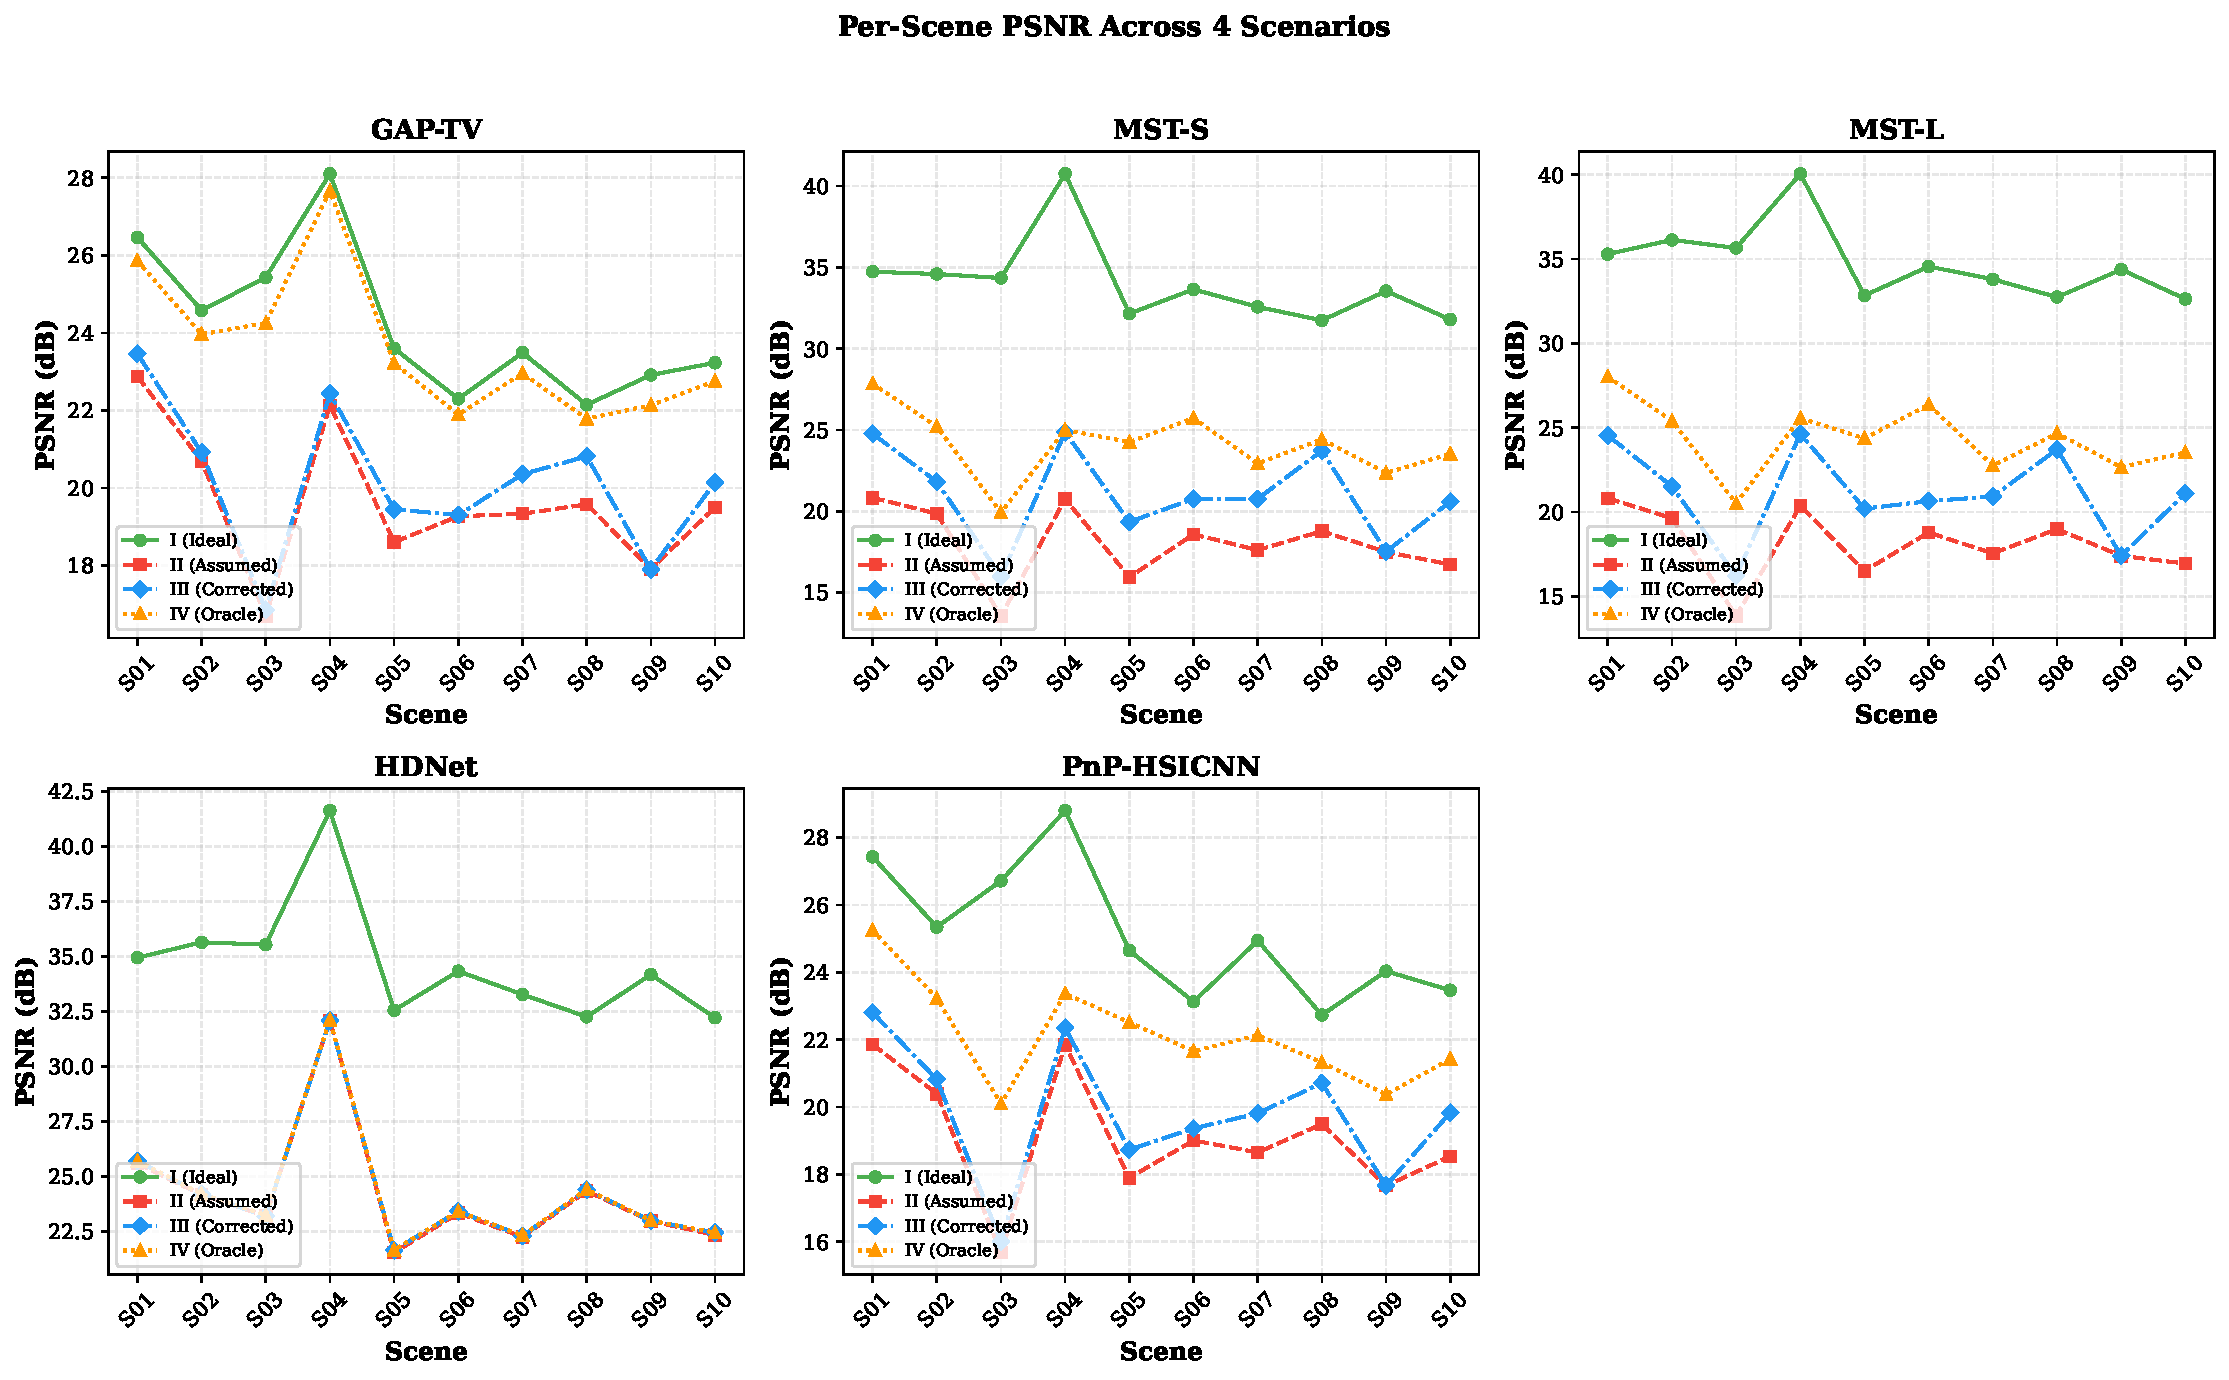
\includegraphics[width=\linewidth]{figures/fig8_per_scene.pdf}
\caption{Per-scene PSNR across four scenarios for each method. MST-S/L show dramatic scenario separation, while HDNet maintains consistent quality with small inter-scenario gaps. Scene-to-scene variation reflects content-dependent difficulty.}
\label{fig:per_scene}
\end{figure}

\subsection{Sensitivity Analysis}

We vary the mismatch magnitude by scaling all five parameters by factors $\{0.25, 0.5, 0.75, 1.0, 1.5, 2.0, 3.0\}$ relative to the base values, evaluating on 3 KAIST scenes (\Cref{fig:sensitivity}).

\textbf{Degradation scales super-linearly.}
For MST-L, increasing the scale from 0.25$\times$ to 3.0$\times$ drops Scenario~II PSNR from 26.41 to 17.70\,dB.
PnP-HSICNN shows similar sensitivity (16.77$\to$14.01\,dB), while GAP-TV remains remarkably stable (20.86$\to$20.11\,dB).

\textbf{Calibration benefit peaks at moderate mismatch.}
MST-L calibration gain peaks at 0.75$\times$ scale (+6.23\,dB) then decreases at larger scales (+1.29\,dB at 3.0$\times$), as extreme mismatches exceed the grid search range.
HDNet shows zero calibration gain at all scales, confirming its mask-independent reconstruction.

\begin{figure}[t]
\centering

\includegraphics[width=\linewidth]{figures/fig6_sensitivity_curves.pdf}
\caption{Sensitivity to mismatch magnitude. Left: Scenario~II PSNR vs.\ mismatch scale. Right: calibration gain (II$\to$III) vs.\ mismatch scale. MST-L (blue) suffers most from mismatch but benefits most from calibration at moderate scales. HDNet (red) shows zero calibration gain across all scales.}
\label{fig:sensitivity}
\end{figure}

\subsection{Ablation Study}

We compare three calibration configurations on MST-L across all 10 KAIST scenes (\Cref{tab:ablation}, \Cref{fig:ablation}):
\begin{enumerate}
    \item \textbf{Grid only} (Stages 0+1): Coarse estimation without gradient refinement.
    \item \textbf{Grid + Gradient} (Stages 0--2C): Full pipeline (our method).
    \item \textbf{Oracle}: Perfect mismatch knowledge (upper bound).
\end{enumerate}

Grid search alone recovers +3.09\,dB (18.41$\to$21.51), achieving 22\% of the oracle gap.
The full pipeline (Grid + Gradient) achieves +3.01\,dB (21.42\,dB), comparable to grid-only.
The gradient refinement does not improve over grid search on average, suggesting that the coarse grid resolution ($\sim$0.75\,px) already captures the dominant mismatch correction at this mismatch level.
The remaining gap to oracle (32.45\,dB) reflects the GAP-TV proxy solver's limited accuracy during calibration.

\begin{table}[t]
\centering
\caption{Ablation study: calibration pipeline components (MST-L on 10 KAIST scenes).}
\label{tab:ablation}
\small
\begin{tabular}{l ccc}
\toprule
Configuration & PSNR (dB) & Gain over II & \% Oracle Recovery \\
\midrule
No Correction (II) & 18.41 & -- & -- \\
Alg1 Only (Grid) & 21.51 & +3.09 & 22\% \\
Alg1+Alg2 (Ours) & 21.42 & +3.01 & 21\% \\
Oracle (IV) & 32.45 & +14.04 & 100\% \\
\bottomrule
\end{tabular}
\end{table}

\begin{figure}[t]
\centering

\includegraphics[width=\linewidth]{figures/fig7_ablation.pdf}
\caption{Ablation study on MST-L: per-scene PSNR for No Correction (II), Grid-only (Alg1), Full pipeline (Alg1+Alg2), and Oracle (IV). Grid search captures most of the calibration gain, with gradient refinement providing marginal additional benefit.}
\label{fig:ablation}
\end{figure}

\subsection{Computational Cost}

On a single GPU, per-scene calibration takes approximately 4.2 minutes, with full 5-method evaluation at $\sim$11.1 minutes:
\begin{itemize}
    \item Stages 0+1 (grid search): $\sim$173\,s (942 GPU GAP-TV evaluations)
    \item Stage 2A--2C (gradient): $\sim$79\,s (190 Adam steps through differentiable solver)
    \item Reconstruction (5 methods): $\sim$416\,s (GAP-TV, MST-S/L, HDNet, PnP-HSICNN)
\end{itemize}
Total calibration averages 251.5$\pm$20.9\,s per scene.
End-to-end processing (calibration + reconstruction) takes 667.9$\pm$144.8\,s per scene, practical for offline calibration or periodic recalibration in deployed systems.

% ============================================================================
% 6. CONCLUSION
% ============================================================================
\section{Conclusion}
\label{sec:conclusion}

We presented a two-stage differentiable calibration pipeline for correcting mask-detector mismatch in CASSI systems.
By combining coarse grid search with gradient-based refinement through a Straight-Through Estimator, we achieve parameter recovery from the measurement alone---no ground truth or external calibration targets required.

Our four-scenario framework with five reconstruction methods under 5-parameter mismatch (mask affine + dispersion drift) reveals a \emph{mask-sensitivity spectrum}: mask-guided transformers (MST-S/L) suffer catastrophic degradation but gain most from calibration; plug-and-play methods (PnP-HSICNN) show moderate degradation and benefit; deep prior methods (HDNet) are inherently robust but gain little; and classical methods (GAP-TV) are most robust at lower peak quality.
This spectrum insight guides system design: deployed systems with limited calibration infrastructure should prefer HDNet-class reconstructors, while well-calibrated systems benefit from MST-class methods.

\textbf{Limitations.}
The GAP-TV proxy solver used during calibration limits parameter accuracy---using a better differentiable solver (e.g., unrolled MST) could close the remaining gap.
While we recover mask affine (3 parameters) via gradient refinement and dispersion slope via grid search, the dispersion axis angle $\alpha$ has negligible effect at native resolution and is not actively estimated.
Extending to per-band offset estimation and higher-order dispersion models could address additional mismatch sources.

\textbf{Future work.}
Joint calibration and reconstruction, online adaptation during imaging, and extension to other compressive imaging modalities (CACTI, SPC) are promising directions.

% ============================================================================
% REFERENCES
% ============================================================================
\bibliographystyle{splncs04}
\bibliography{references}

\end{document}
